% Latex template for submission to the 16th International Meeting on Fully 3D Image Reconstruction 
% in Radiology and Nuclear Medicine (Fully3D 2021)
%
% Author: G.Schramm
% Date:   Oct 2020
%
% In case you encouter problems, you can raise a github issue here:
% https://github.com/gschramm/fully3d_2021_templates/issues

\documentclass[11pt,twocolumn,twoside]{article}
\usepackage{fully3d}

%%%%%% add your extra packages here (if needed)                                       %%%%%
%%%%%% before, have a look which packages are already imported by the fully3d package %%%%%
%\usepackage{mypackage}


%%%%% your bibtex file that contains the bibtex entries here %%%%%
%%%%% please include DOIs in the bibtex entries if possible  %%%%%
\addbibresource{mybib.bib}
\AtBeginBibliography{\footnotesize}

\begin{document}


%-------------------------------------------------------------------------------------------
%%%%% add your title here %%%%%
\title{A LaTex Template for a Fully3D 2021 submission} 

%%%%% add authors and affiliations here %%%%%
\author[1]{\small First~Author}
\author[1,2]{\small Second~Author}
\author[2]{\small Third~Author}

\affil[1]{Department of Nuclear Medicine,
          University of Reconstruction, City, Country}

\affil[2]{Department of Radiology,
          Recon University, City, Country}

%%%%% don't change these 2 lines %%%%%
\maketitle
\thispagestyle{fancy}



%-------------------------------------------------------------------------------------------
%%%%% add your summary (abstract) here               %%%%%%
%%%%% use footnotesize for this section              %%%%%%
%%%%% please stick to the customabstract environment %%%%%% 


\begin{customabstract}
Add your abstract here. This abstract can be slightly longer than the very short 
150 words abstract that you have to enter in the submission system and that is used 
for the program. 
\end{customabstract}


%-------------------------------------------------------------------------------------------
%%%%% main text                                                %%%%%    
%%%%% remove the dummy content and put your own content here   %%%%% 
%%%%% feel free to choose your own section titles              %%%%% 
%%%%% you don't need to put the content in a separate tex file %%%%%

% dummy_content.tex shows how to add sections, figures, tables, formulas, and references
% remove the following line, it just add dummy content
\section{Introduction}

\textbf{\color{red}Submission rules}
\begin{itemize}
\color{red}
\item submission only in pdf format
\item two column format
\item font size 11 for main text, abstract and references can use font size 9 (footnotesize in Latex)
\item maximum 4 A4 pages including everything (strict limit)
\item In addition: prepare short abstract (max 150 words) to be entered in the online submission system. 
      This will only be used for the program. 
      It will not be used for the review process nor for the final proceedings.
\end{itemize}

\lipsum[2-5]


\section{Materials and Methods}

This is how you add references \cite{Doe2020}, \cite{Deen2019}.

% example equation
And this is a dummy equation
\begin{equation}
I_\alpha = \int_0^\alpha f(x) dx
\end{equation}

% example two column figure (use figure instead of figure* for one column figure)
\begin{figure*}
  \centering
  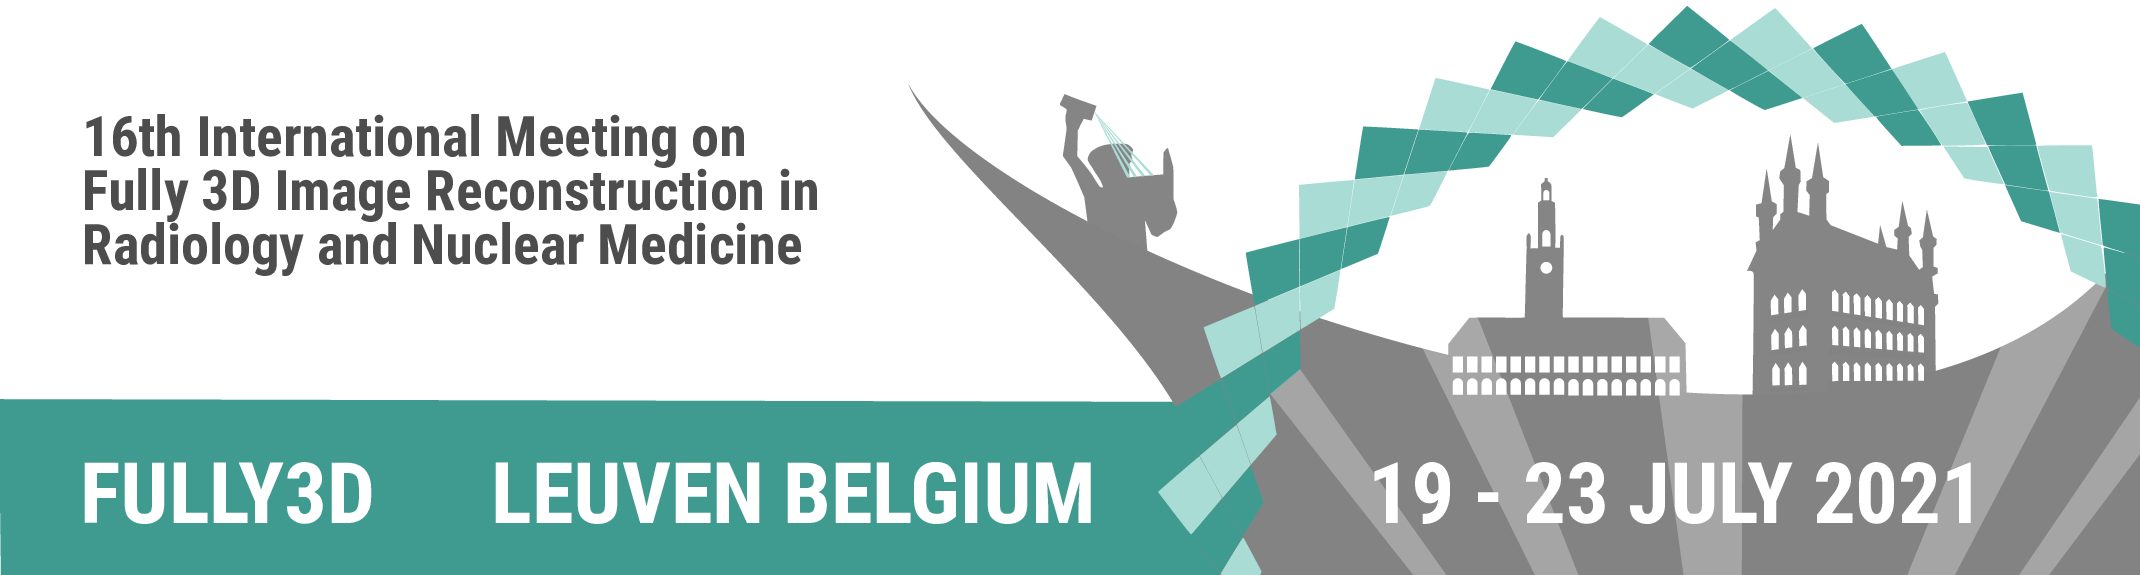
\includegraphics[width=1.0\textwidth]{./fig1.pdf}
  \caption{This a dummy figure to be replaced.}
  \label{fig:dummyfigure}
\end{figure*}

Figure \ref{fig:dummyfigure} shows how to include a figure.
Table \ref{tab:dummytable} shows how to include a table.

\bigskip

\lipsum[2-7]

\section{Results}
\subsection{Simulation results}

\lipsum[2-3]

\subsection{Other results}
\lipsum[2-3]

% example table
\begin{table}
  \centering
  \begin{tabular}{lrrr}
  \toprule
  $\alpha$   & $\beta$ & $\gamma$ & $\delta$ \\
  \midrule
  A          & 1       & a        & 3        \\
  B          & 2       & b        & 2        \\
  C          & 3       & c        & 1        \\
  \bottomrule
  \end{tabular}
  \caption{This is a dummy table to be replaced.}
  \label{tab:dummytable}
\end{table}



\section{Discussion}
\lipsum[2-9]


\section{Conclusion}
\lipsum[2]





%-------------------------------------------------------------------------------------------
\printbibliography

\end{document}
